
\begin{figure}[h]
  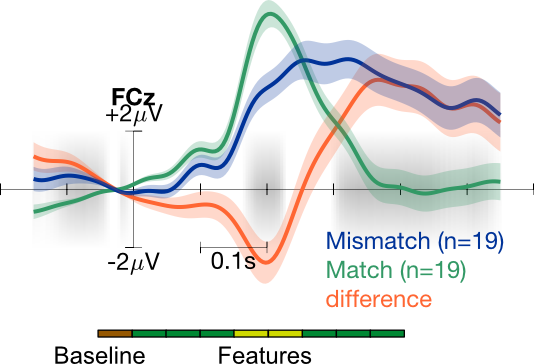
\includegraphics[width=\textwidth]{figures/erp_FCZ_diff_delay.png}
  \caption{Grand-average ERP (n = 19) of projected source mixtures at electrode FCz with significant class differences marked in grey. Bottom: Time windows used to compute features for classification (all greens). Windows in light green indicate time windows of interest for classifier source localization.}
  \label{erp}
\end{figure}

\subsection{77 \% Classification Accuracy Detecting VR Glitches using ERPs}

We found significant differences between match and mismatch trials in the grand-average event-related potential (ERP) at several scalp locations, see \ref{lda_loc} a showing the ERP at electrode `FCz' for an example. Hence, we reproduced our previous findings in \citet{Gehrke2019-og} with an altered processing pipeline. At electrode `FCz', amplitude differences at 200 ms indicated a significant difference between mismatch, i.e. the VR glitch condition and the matching trials ($t_{18} = -5.34, p < .001$). Differences were observed most strongly in the 150-280 ms time window, at 250 ms and in later windows starting at 350 ms, see figure \ref{lda_loc} a.

To assess the potential for single-trial online applications, a discriminative classification system was cross-validated. The system, using windowed mean ERP features, succeeded in detecting VR glitches. Mismatch and match trials were correctly labeled to the corresponding class with an average accuracy of ~77 percent ($SD = 9.12$). The classification accuracy exceeded chance level at \textasciitilde 56 percent, $t_{(18)} = 42.1, p < .001$. 

\begin{figure}
  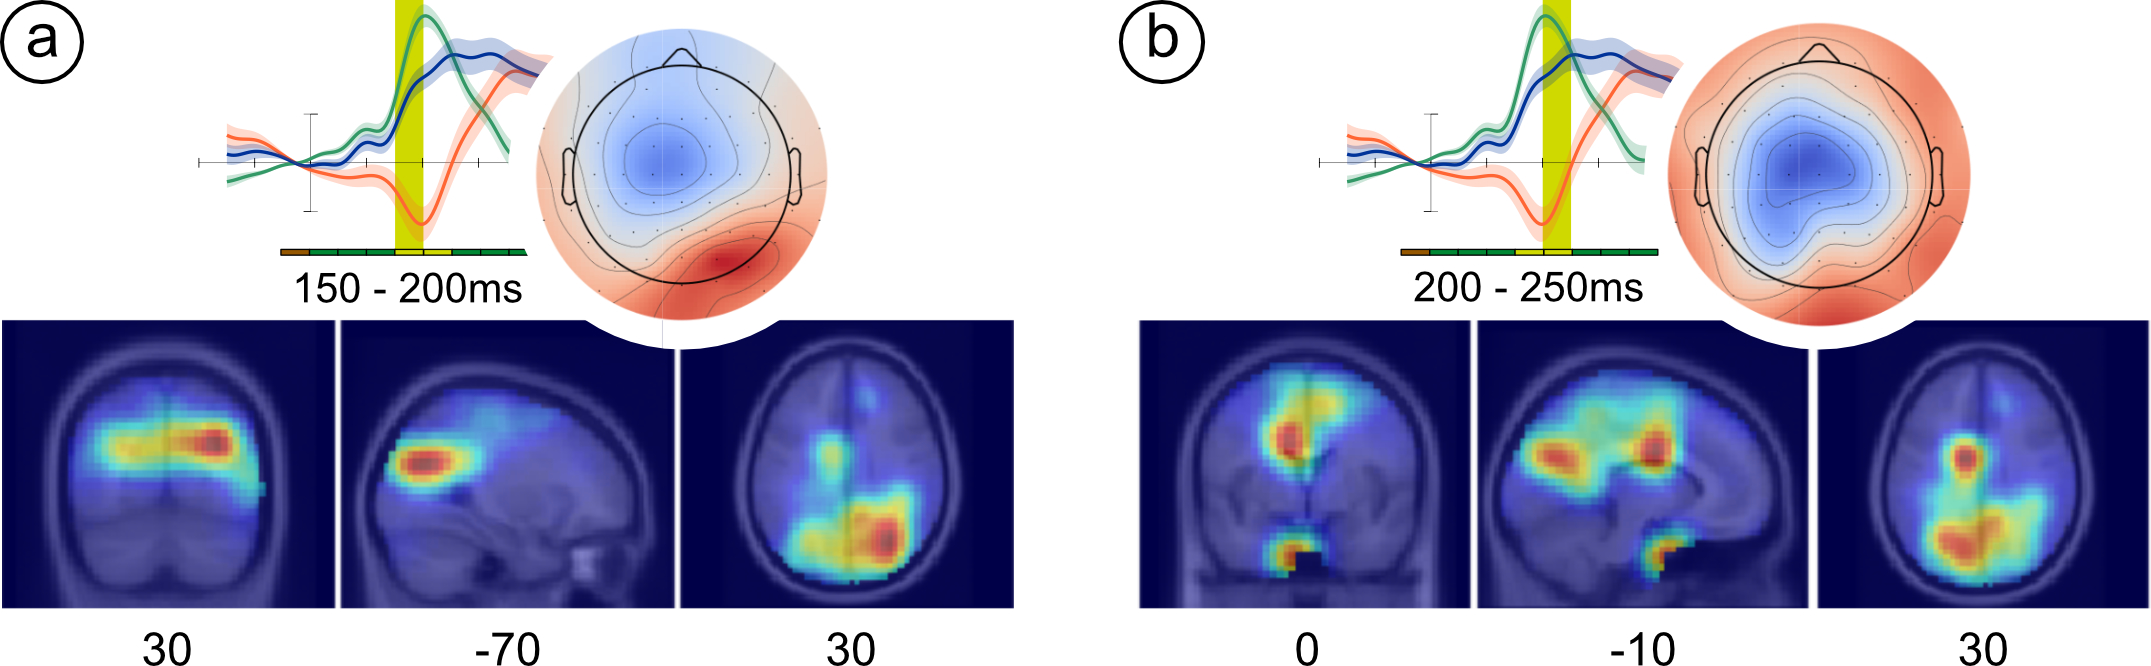
\includegraphics[width=\textwidth]{figures/fig_localization.jpg}
  \caption{An LDA classifier was trained on eight windowed means of 50 ms size from 0 to 400 ms following the cube touch, see figure \ref{erp} bottom. Two classes of synchronous and asynchronous trials were labeled for training and cross-validation. \textbf{A, B} Scalp maps of difference-between-classes activity for the 4th (150-200) and 5th (200-250ms) time windows and the equivalent source localization (MNI coordinates).}
  \label{lda_loc}
\end{figure}

\subsubsection{Classification Driven by Midline Cingulate and Occipital EEG Sources}

Next, we investigated which EEG sources contributed maximally to the classification to draw conclusions about the cortical origin of the discriminatory signal. This source reconstruction served two purposes with regards to the system's applicability as robust neural interface technology: (1) Asserting that the classifier did not rely \textit{primarily} on artifact EEG sources, and (2) to gain additional information about the contributing brain regions to allow interpretations about cognitive processing.

In the fourth time window (150 - 200 ms, see the light green shaded segment in \ref{lda_loc} a) classifications were driven primarily by activity originating in right lateral parieto-occipital cortical sources (BA19; MNI: x = 30, y = -70, z = 30). In the following time-window (200 - 250 ms, light green shading in \ref{lda_loc} b) the classification signal draw from distributed source activity in occipital areas as well as from sources located in anterior midline cingulate gyrus (near BA23; MNI: x = 0, y = -10, z = 30). Some ocular sources were not classified as such by our automated processing pipeline and carried information relevant to classification in this time window of interest.